\chapter{Architettura MyData}
\label{capitolo3}
\thispagestyle{empty}

\noindent Al fine di comprendere appieno le scelte effettuate all’interno del progetto, si evidenziano brevemente le componenti e la struttura del modello \textit{MyData} \cite{githubmydatastack}. 

\section{Entit\`a Fondamentali}
L’architettura di \textit{MyData} si costruisce su quattro componenti base: l’utente finale, detto anche \textit{Account Owner}, l’operatore \textit{MyData}, o \textit{Operator}, e due generiche entit\`a che, da una parte, “producono” dati, e, dall’altra, li “consumano”. Esse sono definite rispettivamente \textit{Source} e \textit{Sink}. Mentre i ruoli di Account Owner e di Operator sono generalmente statici, quelli di Source e Sink sono fortemente variabili nel tempo e si possono applicare anche ad entit\`a molto diverse fra loro, poich\'e definiti con un alto livello di astrazione. Convenzionalmente, si pu\`o identificare un servizio come “consumatore” di dati, mentre l’account dell’utente pu\`o essere un “produttore” di dati personali. In \textit{MyData}, \`e possibile altres\`i che un servizio occupi entrambi i ruoli, o anche che l’\textit{Operator} stesso rientri in questa classificazione quando si trova a compiere operazioni sui dati.

Il ruolo di \textit{Operator} comprende operazioni di vario genere fra i quali vi sono la gestione degli utenti, dei servizi e delle interazioni che avvengono fra le due parti. Esso si occupa anche di gestire l’Audit Log di tutte le operazioni che coinvolgono tali interazioni.

\section{Service Registry, Service Linking}
Con \textit{Service Registry} viene indicata quella parte dell’\textit{Operator} che contiene un database di tutti i servizi registrati presso l’operatore stesso. Esso contiene anche la funzionalit\`a di \textit{Service Discovery}, utilizzata dagli utenti per trovare nuovi servizi da utilizzare. In particolare, gli utenti possono venire a conoscenza di un nuovo servizio tramite un suggerimento, calcolato in base a corrispondenze fra caratteristiche dell’utente e del servizio, oppure tramite ricerca diretta.

Ogni nuovo servizio che vuole essere utilizzabile all’interno dell’architettura \textit{MyData} deve quindi sottoporsi ad una procedura di registrazione al termine della quale, in caso di successo, viene inserito all’interno del \textit{Registry}.

Durante questa procedura, il servizio deve fornire almeno una descrizione del suo comportamento in formato machine-readable e human-readable: la prima permette a procedure automatiche un'elaborazione corretta di suggerimenti, la seconda \`e rivolta direttamente all’utente finale.

L’iscrizione di un utente presso un servizio avviene tramite un processo chiamato \textit{Service Linking}, in cui l’Operatore \textit{MyData} si occupa di realizzare un'identificazione mutua delle parti. Tutti i token e le firme digitali scambiate durante il procedimento sono espresse in notazione JSON.

Al termine del \textit{Service Linking} viene prodotto un \textit{Service Link Record}, necessario per ogni futura interazione fra l’utente ed il servizio.

\subsection{OAuth 2.0}
\begin{figure} [h]
	\centering
	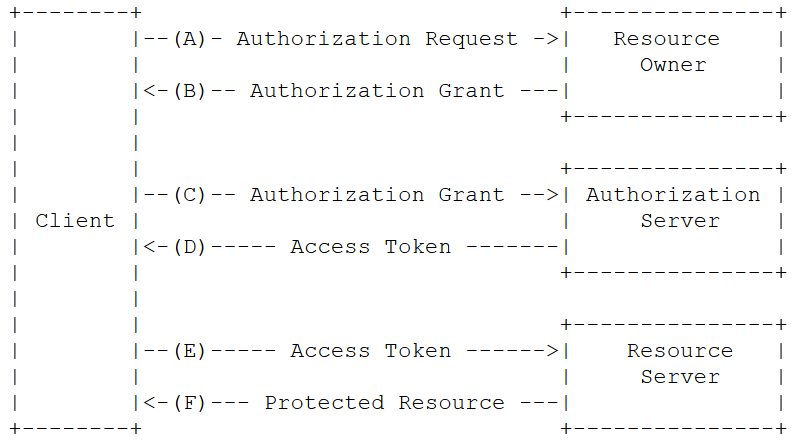
\includegraphics[width=0.6\linewidth]{pictures/OAuthAbstractProtocolFlow.png}
	\caption{RFC 6749, OAuth 2.0 Abstract Protocol Flow}
	\label{fig:OAuthAbstractProtocolFlow}
\end{figure}
OAuth \`e un protocollo per il controllo dei flussi di autorizzazioni fra mobile applications, desktop applications, dispositivi mobili, ecc. \cite{oauth}. Se ne d\`a un breve accenno in questa sede in quanto esso viene preso come esempio di implementazione di \textit{Service Linking} all’interno delle specifiche di \textit{MyData} \cite{githubmydatastack}.

Le entit\`a coinvolte nel protocollo di autorizzazione le seguenti:
\begin{itemize}
	\item Un’applicazione Client, che richiede l’accesso ad un account utente;
	\item Un \textit{Resource Owner}, spesso coincidente con l’utente finale, che accorda o nega l’accesso ad una porzione del suo account;
	\item Un \textit{Resource Server} dove sono memorizzati gli account, che espone determinate API per l’accesso e discrimina le richieste legittime in base ad \textit{access token};
	\item Un \textit{Authorization Server} che emette gli \textit{access token} dopo aver provato l’identit\`a dell’utente finale, e solo in caso quest’ultimo abbia acconsentito all’utilizzo dei suoi dati. Pu\`o coincidere con il \textit{Resource Server}.
\end{itemize}
\`E facilmente riscontrabile un’analogia con le entit\`a descritte all’interno dell’architettura \textit{MyData}, ad esempio fra \textit{Sink} e applicazione Client, fra \textit{Source} e \textit{Resource Server}, fra \textit{Account Owner} e \textit{Resource Owner}, e infine fra l’Operatore \textit{MyData} e \textit{Autorization Server}.

In figura \ref{fig:OAuthAbstractProtocolFlow} \`e mostrato il flusso di autorizzazioni implementato dal protocollo OAuth 2.0, dal quale \`e stato preso spunto per la definizione di \textit{Service Linking} e delle interazioni in \textit{MyData}. Le analogie possono essere riassunte all’interno dei seguenti punti:
\begin{itemize}
	\item I punti (A) e (B) corrispondono alla registrazione di un utente presso un servizio; questo stato viene spesso indicato come precondizione per il \textit{Service Linking} all’interno della documentazione \textit{MyData}.
	\item I punti (C ) e (D) riassumono i passi che l’Operatore compie per identificare il servizio, emettere ID surrogati e \textit{token key} e svolgere le operazioni di autenticazione e firma da parte di \textit{Account Owner} e del servizio stesso.
	\item i punti (E) e (F) descrivono come avviene effettivamente il recupero dei dati una volta ottenuta l’autorizzazione necessaria. In \textit{MyData} ci\`o corrisponde alla “connessione dati” che si instaura fra \textit{Source} e \textit{Sink}.
\end{itemize}
Vista la forte analogia con \textit{MyData}, in fase di Progettazione (capitolo \ref{capitolo5}) ho scelto di prendere spunto dal protocollo OAuth 2.0 al momento di definire un algoritmo per l’autenticazione e le relazioni fra le parti. 

\section{Autorizzazioni e Consent}
\label{sec:MD-AuthConsent}
Come specificato dal GDPR, ogni operazione svolta sui dati personali di un utente deve essere stata autorizzata dallo stesso tramite un permesso che acquista in questo contesto una valenza legale.

La funzione di un permesso, o Consent, \`e particolarmente rilevante: definisce quali dati possono essere utilizzati e in che modalit\`a, e identifica le entit\`a \textit{Source} e \textit{Sink} fra le quali avviene lo scambio. Il processo di \textit{Service Linking} deve essere stato completato con successo affinch\'e sia possibile fare richiesta di autorizzazione, e ci\`o viene verificato tramite ispezione del \textit{Service Link Record}.

Il ruolo dell’\textit{Operator} in questa situazione \`e quello di recuperare le informazioni corrispondenti al servizio presso il \textit{Service Registry}: queste vengono presentate all’utente che decide se acconsentire o meno al processamento di un determinato insieme di dati da parte di un servizio specificato. \`E possibile per l’utente chiedere una ridefinizione delle richieste del servizio, ma non al di sotto del limite previsto per un corretto svolgimento del servizio stesso. Tale insieme di dati viene identificato mediante un \textit{Resource Set Identifier}, che permette a \textit{Source} e \textit{Sink} di identificare precisamente le risorse da trasmettere.

Nel caso la procedura di autorizzazione si concluda con successo, viene prodotto un \textit{Consent Record} che contiene tutte le specifiche negoziate fra le parti insieme agli identificatori dell’utente e del servizio. Esso viene memorizzato all’interno dell’account, ma \`e possibile che il servizio o l’Operatore ne facciano richiesta successivamente. 

Per dare la possibilit\`a all’utente di ritirare il permesso accordato, un Consent ha tre stati possibili: \textit{Active}, \textit{Disabled} e \textit{Withdrawn}. Il primo \`e lo stato standard di funzionamento, in cui l’accesso ai dati \`e consentito; si hanno poi gli stati “disabilitato” e “ritirato”, in cui l’accesso \`e impedito. Nel caso in cui il permesso sia stato ritirato \`e necessario provvedere all’emissione di una nuova autorizzazione, mentre in caso di stato disabilitato, \`e possibile attuare un cambiamento di stato, riportandolo al valore attivo.

Questo protocollo di autorizzazione all’utilizzo dei dati rispetta quindi quanto affermato dal GDPR, poich\'e il permesso viene dato volontariamente e in modo chiaro. Non \`e ambiguo, \`e informato, grazie alla specifica delle risorse necessarie, ed \`e possibile ritirarlo in ogni momento.

\subsection{Kantara Consent Notice Receipt Specification}
All’interno della documentazione di \textit{MyData} \cite{githubmydatastack} viene indicato il documento di specifica \textit{Consent Notice Recipt Specification} (CNRS) elaborato da Kantara \cite{kantaraconsent} come esempio di \textit{Consent Record}. Il contesto di sviluppo alla base di questo documento \`e simile a quello di \textit{MyData}, descritto nei capitoli \ref{Introduzione} e \ref{capitolo2}, e consiste nell’offrire agli utenti la possibilit\`a di venire a conoscenza dell’uso che viene fatto dei propri dati e di poter intervenire attivamente nella sua gestione.

Pertanto, l’obiettivo del CNRS \`e quello di definire uno standard di implementazione per record di autorizzazioni e transazioni di dati, al fine di supportare l’interoperabilit\`a fra sistemi diversi, offrire una prova credibile di autorizzazione ricevuta e dare il via a “buone pratiche” e consuetudini coerenti con il rispetto della privacy e la tracciabilit\`a delle trasmissioni di dati.

All’interno del documento viene dettagliata la terminologia specifica del settore relativo a privacy e autorizzazioni, ad esempio mediante la definizione del termine “\textit{Consent}”, che riporto di seguito perch\'e particolarmente rilevante all’interno del contesto:
\begin{quote}
A Personally identifiable information (PII) Principal’s freely given, specific and informed agreement to the processing of their PII.
\end{quote}
Altri esempi comprendono la definizione di \textit{Personally Identifiable Information} e \textit{Consent Recipt}.

Successivamente, viene descritta la struttura dati proposta come standard di \textit{Consent Receipt}, dettagliando ogni campo presente al suo interno. Ho preso spunto da questo documento al momento di realizzare i \textit{Consent} all’interno del gestore di dati personali (sottosezione \ref{subsec:P-ServiceConsentDataConsent}).

\subsection{User Managed Access}
\cite{uma}

\section{Personal Data Storage}
Nonostante non venga dato un peso rilevante a questa componente all’interno delle specifiche \textit{MyData} \cite{githubmydatastack}, non \`e possibile prescindere dall’esistenza di un database che mantenga tutti i dati relativi ad un \textit{Account Owner}. Non si tratta infatti solo di dati personali, ma di ogni dato utilizzato da un generico servizio o ad esempio inserito volontariamente dall’utente.

Non \`e specificato se il Personal Data Storage (spesso chiamato anche Personal Data Vault) faccia parte dell’ecosistema dell’operatore: ci\`o \`e possibile, ma non sono da escludere implementazioni alternative che prevedono il salvataggio delle informazioni presso il dispositivo dell’utente o in un database sicuro.

L’accesso ai dati contenuti all’interno del Personal Data Storage \`e possibile solo in presenza di un adeguato \textit{Consent Record}, ma le modalit\`a di accesso non vengono regolamentate in maniera dettagliata. Si parla infatti genericamente di “Data API”, con le quali un \textit{Sink} ottiene (in caso di richiesta legittima) un determinato \textit{Resource Set} da un \textit{Source}.

Poiché l’applicazione Mobility Profile \`e stata sviluppata in un secondo momento rispetto alla prima pubblicazione delle specifiche tecniche suddette, si \`e provveduto all’interno della relativa documentazione \cite{githubmobilityprofilespecification} ad aggiungere una breve menzione del Personal Data Storage, spiegando il suo ruolo all’interno dell’applicazione.

Dall’analisi del codice disponibile sul repository Github \cite{githubmobilityprofile} \`e emerso che i dati personali vengono mantenuti all’interno del dispositivo mobile e gestiti attraverso un database relazionale \cite{ormSugar}. Questa implementazione differisce leggermente da quella proposta inizialmente, in quanto la computazione avviene localmente ai dati invece che presso il servizio. All’interno del progetto del gestore di dati personali ho scelto di restare aderente alle prime specifiche di \textit{MyData} \cite{githubmydatastack}. Questa problematica viene analizzata pi\`u in dettaglio prima in fase di Analisi (sezione \ref{sec:A-PDS}) e successivamente in fase di Progettazione (sottosezione \ref{subsec:P-PDV}).